% id: 0142
% book: RPM 중3-2 수학 · 01 삼각비
% section: 중단원 마무리하기
% figure: crop:fig-0142.png
% answer: ①
% answer_source: 답지
% variant_level: 0 (원본 전사)
% 이 파일은 build.mjs 가 items.json 에서 만든다. 고칠 때는 items.json 을 고친다.
다음 삼각비의 표를 이용하여 $\sin 47^\circ+\cos 50^\circ-\tan 48^\circ$의 값을 구하면?
\par\smallskip\begin{center}\setlength{\dmfigw}{240.7pt}\ifdim\dmfigw>\linewidth\setlength{\dmfigw}{\linewidth}\fi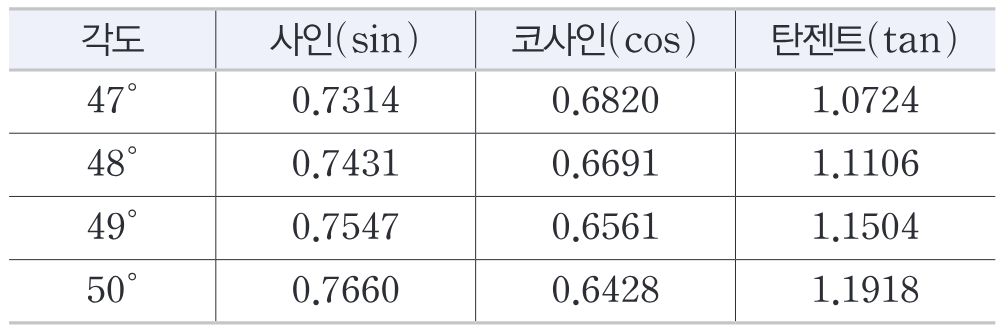
\includegraphics[width=\dmfigw]{figures/fig-0142.png}\end{center}
\dmchoicesauto{}{$0.2636$}{$0.2769$}{$0.3016$}{$0.3374$}{$0.3410$}
